\chapter{Progettazione di Basi di Dati}

Progettare una basi di dati vuole dire progettare la struttura dei dati e le applicazioni:\ è l'attività più importante.\
Per progettare i dati al meglio è necessario che i dati siano un modello fedele del dominio del discorso.

\begin{definition}
	Un modello astratto è la rappresentazione formale di idee e conoscenze relative a un fenomeno.\
\end{definition}

\noindent Aspetti di un modello:
\begin{itemize}
	\item il modello è la rappresentazione di certi fatti;
	\item la rappresentazione è data con un linguaggio formale;
	\item il modello è il risultato di un processo di interpretazione, guidato dalle idee e conoscenze possedute dal soggetto che interpreta.
\end{itemize}
La stessa realtà può utilmente essere modellata in modi diversi e a diversi livelli di astrazione.\

\begin{figure}[H]
	\centering
	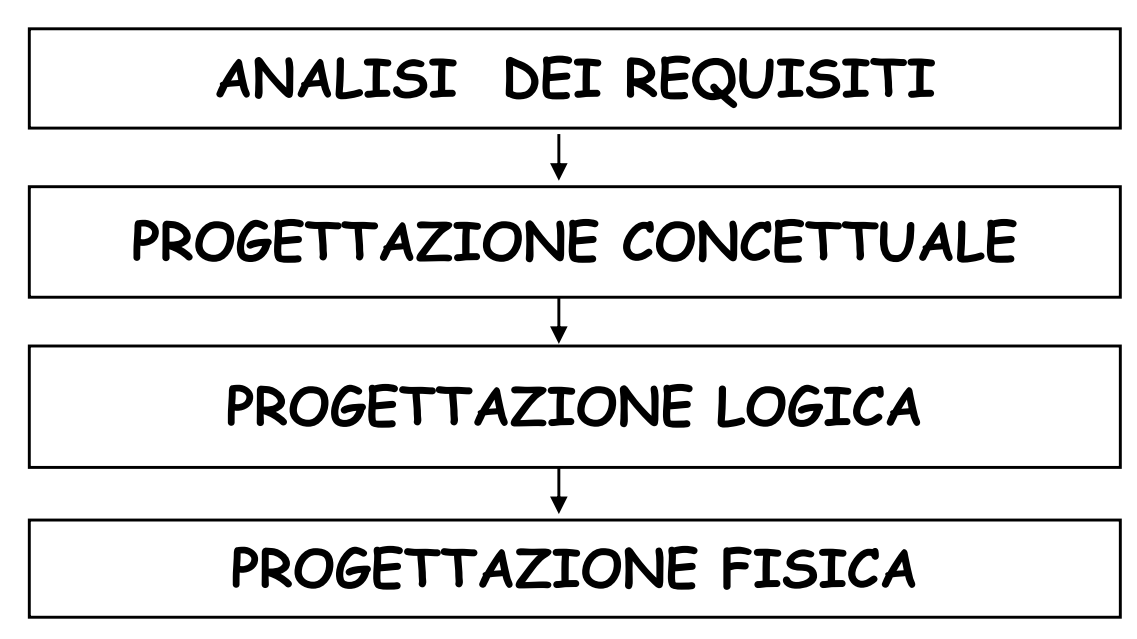
\includegraphics[width=0.5\textwidth]{immagini/Progettazione.png}
\end{figure}
\noindent Ciascuna di queste fasi è centrata sulla modellazione.\
La modellazione verrà discussa quindi con riferimento alla problematica della progettazione delle basi di dati.\

\begin{figure}[H]
	\centering
	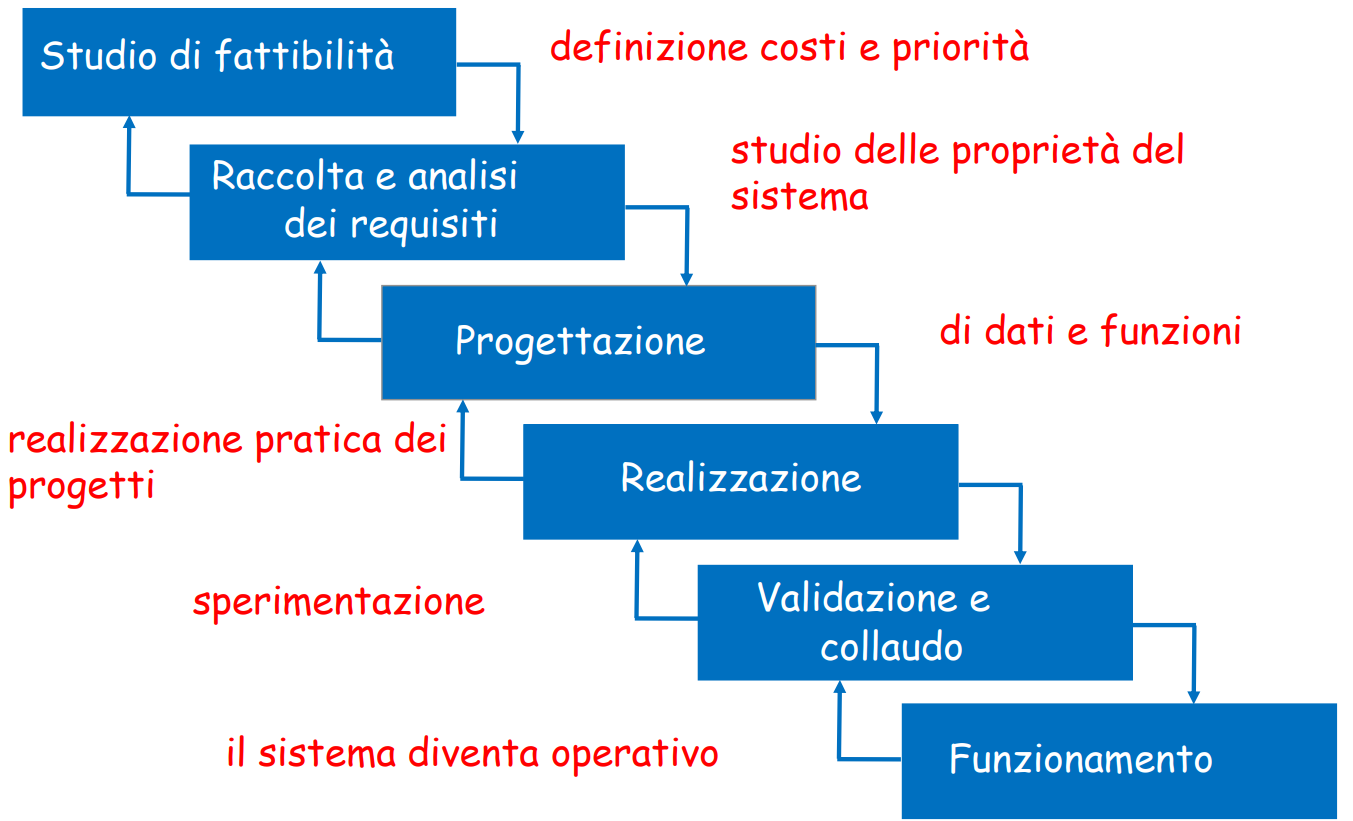
\includegraphics[width=0.8\textwidth]{immagini/Progettazione2.png}
\end{figure}
\noindent Per garantire prodotti di buona qualità è opportuno seguire una \textbf{metodologia di progetto} con:
\begin{itemize}
	\item Articolazione delle attività in fasi (\textbf{decomposizione})
	\item Criteri di scelta (\textbf{strategie})
	\item \textbf{Modelli} di rappresentazione
	\item \textbf{Generalità} rispetto al problema di studio e agli strumenti a disposizione
	\item \textbf{Qualità} del prodotto
	\item \textbf{Facilità} d'uso
\end{itemize}

\subsubsection{Modello dei dati}
Insieme di costrutti utilizzati per organizzare i dati di interesse e descriverne la dinamica.\
Componente fondamentale:\ \textbf{meccanismi di strutturazione} (o costruttori di tipo).\
Come nei linguaggi di programmazione esistono meccanismi che permettono di definire \textbf{nuovi tipi}, così ogni modello dei dati prevede alcuni costruttori.\
Ad esempio, il modello relazionale prevede il costruttore relazione, che permette di definire insiemi di record omogenei.

\subsubsection{Aspetti del problema}
Quale conoscenza del dominio del discorso si rappresenta?\
Aspetto \textbf{ontologico} (studio di ciò che esiste):\ ciò che si suppone esistere nell'universo del discorso e quindi sia da modellare.

\noindent Con quali meccanismi di astrazione si modella?\
Aspetto \textbf{logico}.\

\noindent Con quale linguaggio formale si definisce il modello?\
Aspetto \textbf{linguistico}.\

\noindent Come si procede per costruire un modello?\
Aspetto \textbf{pragmatico}:\ metodologia (insieme di regole finalizzate alla costruzione del modello informatico) da seguire nel processo di modellazione

\section{Aspetto Ontologico: cosa si modella}
\begin{itemize}
	\item Conoscenza concreta:\ i fatti.
	\item Conoscenza astratta:\ struttura e vincoli sulla conoscenza concreta.
	\item Conoscenza procedurale, comunicazioni:
	      \begin{itemize}
		      \item le operazioni di base, le operazioni degli utenti;
		      \item come si comunicherà con il sistema informatico.
	      \end{itemize}
\end{itemize}
Nel seguito l'attenzione sarà sulla conoscenza concreta e astratta.

\section{Aspetto Logico: il modello dei dati a oggetti}

Un modello dei dati è un insieme di meccanismi di astrazione per descrivere la struttura della conoscenza concreta.\

Schema:\ la descrizione della struttura della conoscenza concreta e dei vincoli di integrità usando un particolare modello dei dati.

Useremo come notazione grafica una \textbf{variante} dei cosiddetti diagrammi a oggetti o diagrammi ER (Entità-Relazione).\
Nozioni fondamentali:
\begin{itemize}
	\item Oggetto, Tipo di oggetto, Classe
	\item Ereditarietà, Gerarchia fra tipi, Gerarchia fra classi
\end{itemize}

\section{Cosa si modella: la conoscenza concreta}
La \textbf{conoscenza concreta} riguarda i fatti specifici che si vogliono rappresentare:\ le entità con le loro proprietà, le collezioni di entità omogenee e le associazioni fra entità.

\subsection{Conoscenza concreta: entità e proprietà}
Le \textbf{\textit{entità}} sono ciò di cui interessa rappresentare alcuni fatti (o proprietà), per esempio una descrizione bibliografica di un libro, un libro o documento fisico, un prestito, un utente della biblioteca.

Le \textbf{\textit{proprietà}} sono fatti che interessano solo in quanto descrivono caratteristiche di determinate entità, per esempio un indirizzo interessa perché è l'indirizzo di un utente.\
Classificazione delle proprietà:
\begin{itemize}
	\item primitiva/strutturata,
	\item obbligatoria/opzionale,
	\item univoca/multivalore,
	\item costante/variabile,
	\item calcolata/non calcolata.
\end{itemize}

\subsubsection{Conoscenza concreta: collezioni di entità}
Una \textbf{\textit{proprietà}} è una coppia $\langle\mathtt{attributo, valore}\rangle$.

\noindent\textbf{\textit{Tipi di entità}}:\ ogni entità appartiene ad un tipo che ne specifica la natura.\
Ad esempio Antonio ha tipo \texttt{Persona} con proprietà \texttt{Nome:\ string} e \texttt{Indirizzo:\ string}.

\noindent \textbf{\textit{Collezione}}:\ un insieme variabile nel tempo di entità omogenee (dello stesso tipo).\
Ad esempio la collezione di tutte le persone nel dominio del discorso.

\subsubsection{Caratteristiche delle proprietà}

Ogni \textbf{proprietà} ha associato un dominio, ovvero l'insieme dei possibili valori che tale proprietà può assumere:
\begin{itemize}
	\item proprietà \textbf{atomica} se il suo valore non è scomponibile, altrimenti è detta \textbf{strutturata};
	\item proprietà \textbf{univoca} se il suo valore è unico, altrimenti è detta \textbf{multivalore};
	\item proprietà \textbf{totale} (obbligatoria) se ogni entità dell'universo del discorso ha per essa un valore specificato, altrimenti è detta \textbf{parziale} (opzionale).
\end{itemize}
Certi fatti possono essere interpretati come proprietà in certi contesti e come entità in altri.

\subsection{Conoscenza concreta:\ collezioni}
Una \textbf{collezione} è un insieme variabile nel tempo di entità omogenee interessanti dell'universo del discorso.

\subsection{Modellazione a oggetti:\ classi e oggetti}
Ad ogni entità del dominio corrisponde un oggetto del modello.\
\textbf{\textit{Oggetto}}:\ un'entità software con stato, comportamento e identità che modella un'entità dell'universo:
\begin{itemize}
	\item lo \textbf{\textit{stato}} è modellato da un insieme di costanti o variabili con valori di qualsiasi complessità;
	\item il \textbf{\textit{comportamento}} è un insieme di procedure locali chiamate \textbf{metodi} che modellano le operazioni di base che riguardano l'oggetto e le proprietà derivabili da altre.
\end{itemize}
Un \textbf{\textit{oggetto}} può rispondere a dei \textbf{\textit{messaggi}}, restituendo valori memorizzati nello stato o calcolati con una procedura locale.

Una \textbf{classe} è un insieme di oggetti dello stesso tipo, modificabile con operatori per includere o estrarre elementi dall'insieme.

\subsubsection{Tipo oggetto}
Il primo passo nella costruzione di un modello consiste nella \textit{classificazione delle entità del dominio con la definizione dei tipi degli oggetti che le rappre\-sentano}.\

Un \textbf{\textit{tipo oggetto}} definisce l'insieme dei messaggi (interfaccia) a cui può rispondere un insieme di possibili oggetti.\
I \textbf{nomi dei messaggi} sono detti anche attributi degli oggetti.

Nei diagrammi ER i tipi oggetti non si rappresentano, l'attenzione è invece sulle collezioni e sulle associazioni; tuttavia, la rappresentazione grafica di una collezione indica anche gli attributi del tipo oggetto associato.

\subsection{Conoscenza concreta: le associazioni}

Un'\textbf{istanza di associazione} è un fatto che correla due o più entità, stabilendo un legame logico tra di loro.\
Un'associazione $R(X, Y)$ fra due collezioni di entità $X$ ed $Y$ è un insieme di istanze di associazione tra elementi di $X$ e $Y$ che in generale varia nel tempo.

Il prodotto cartesiano ($X \times Y$) è detto dominio dell'associazione.

\subsubsection{Tipi di associazione}

Un'\textbf{associazione} è caratterizzata dalle seguenti proprietà strutturali:\ \textbf{molteplicità} e \textbf{totalità}.

\textbf{Vincolo di univocità}:\ un'associazione $R(X, Y)$ è univoca rispetto a $X$ se per ogni elemento $x$ di $X$ esiste al più un elemento di $Y$ che è associato a $x$, se non vale questo vincolo, l'associazione è multivalore rispetto ad $X$.

\noindent Cardinalità dell'associazione:
\begin{itemize}
	\item $R(X,Y)$ è $(1:N)$ se essa è multivalore su $X$ ed univoca su $Y$.
	\item $R(X,Y)$ è $(N:1)$ se essa è univoca su $X$ e multivalore su $Y$.
	\item $R(X,Y)$ è $(N:M)$ se essa è multivalore su $X$ e multivalore su $Y$.
	\item $R(X,Y)$ è $(1:1)$ se essa è univoca su $X$ e univoca su $Y$.
\end{itemize}
\textbf{Vincolo di totalità}:\ un'associazione $R(X, Y)$ è \textbf{totale} (o suriettiva) su $X$ se per ogni elemento $x$ di $X$ esiste almeno un elemento di $Y$ che è associato ad $x$,  se non vale questo vincolo, l'associazione è \textbf{parziale} rispetto ad $X$.

\subsubsection{Rappresentazione delle associazioni - Associazione binaria senza proprietà}

Un'\textbf{associazione} fra due collezioni C\textsubscript{1} e C\textsubscript{2} si rappresenta con una linea che collega le classi che rappresentano le due collezioni.\
La \textbf{linea} è etichettata con il nome dell'associazione che di solito viene scelto utilizzando un predicato (``soggetto predicato complemento'').\
L'\textbf{univocità} di un'associazione, rispetto ad una classe C\textsubscript{1}, si rappresenta disegnando una freccia singola sulla linea che esce dalla classe C\textsubscript{1} ed entra nella classe C\textsubscript{2}; l'assenza di tale vincolo è indicata da una freccia doppia.\
Similmente, la \textbf{parzialità} è rappresentata con un taglio sulla linea vicino alla freccia, mentre il vincolo di \textbf{totalità} è rappresentato dall'assenza di tale taglio.

\subsubsection{Questioni terminologiche}

\begin{table}[H]
	\centering
	\begin{tabular}{|l|l|}
		\hline
		\textit{Dominio del discorso} & \textit{Modello Informatico} \\\hline\hline
		Entità                        & Oggetto (entity instance)    \\
		Tipo entità                   & Tipo oggetto (entity type)   \\
		Collezione                    & Classe (entity)              \\
		Associazione                  & Associazione (relationship)  \\\hline
	\end{tabular}
\end{table}

\subsubsection{Modello a oggetti:\ le associazioni}

Le associazioni si modellano con un costrutto apposito.\
Possono avere delle proprietà e possono essere ricorsive.\

Le \textbf{associazioni ricorsive} sono relazioni binarie fra gli elementi di una stessa collezione.\
Occorre etichettare la linea non solo con il nome dell'associa\-zione, ma anche con dei nomi per specificare il ruolo che hanno i due compo\-nenti in un'istanza di associazione.\

Per semplicità non daremo una notazione grafica per rappresentare associazioni \textbf{non binarie}.

\subsection{Conoscenza concreta:\ gerarchie di classi}

Spesso le classi di entità sono organizzate in una gerarchia di \textbf{specializzazione}/\textbf{generalizzazione}.\
Una classe della gerarchia minore di altre viene detta \textbf{sottoclasse} (le altre sono superclassi).
Due importanti caratteristiche delle gerarchie:
\begin{itemize}
	\item \textbf{ereditarietà} delle proprietà;
	\item gli elementi di una sottoclasse sono un sottoinsieme degli elementi della \textbf{superclasse}.
\end{itemize}

\subsubsection{Modello a oggetti:\ gerarchia tra tipi oggetto}

Fra i tipi oggetto è definita una relazione di sottotipo \textbf{asimmetrica}, \textbf{riflessiva} e \textbf{transitiva} (relazione di ordine parziale).\

Se $T$ è sottotipo di $T'$, allora gli elementi di $T$ possono essere usati in ogni contesto in cui possano apparire valori di tipo $T'$ (sostituibilità).\
In particolare:
\begin{itemize}
	\item gli elementi di $T$ hanno tutte le proprietà degli elementi di $T'$
	\item per ogni proprietà $p$ in $T'$, il suo tipo in $T$ è un sottotipo del suo tipo in $T'$.
\end{itemize}
La gerarchia può essere semplice o multipla.

\subsubsection{Ereditarietà}

L'ereditarietà (\textit{inheritance}) permette di definire un tipo oggetto a partire da un altro e l'implementazione di un tipo oggetto a partire da un'altra implementazione.\
Normalmente l'eredità tra tipi si usa solo per definire sottotipi, e l'ereditarietà tra implementazioni per definire implementazioni di
sottotipi (ereditarietà stretta); in questo caso gli attributi possono essere solo aggiunti e possono essere ridefiniti solo specializzandone il tipo.

\subsubsection{Sottoinsiemi}

Fra le classi può essere definita una relazione di sottoclasse, detta anche \textbf{sottoinsieme}, con le seguenti proprietà:
\begin{itemize}
	\item È asimmetrica, riflessiva e transitiva.
	\item Se $C$ è sottoclasse di $C'$, allora il \textit{tipo} degli elementi di $C$ è \textit{sottotipo} del tipo degli elementi di $C'$ (vincolo \textbf{intensionale}).
	\item Se $C$ è sottoclasse di $C'$, allora gli \textit{elementi} di $C$ sono un \textit{sottoinsieme} degli elementi di $C'$ (vincolo \textbf{estensionale}).
\end{itemize}
Vincoli su insiemi di sottoclassi:
\begin{itemize}
	\item \textbf{Disgiunzione}:\ ogni coppia di sottoclassi in questo insieme è disgiunta, ovvero è priva di elementi comuni (sottoclassi disgiunte).
	\item \textbf{Copertura}:\ l'unione degli elementi delle sottoclassi coincide con l'insieme degli elementi della superclasse (sottoclassi copertura).
\end{itemize}
Sottoclassi \textbf{scorrelate} non richiedono il vincolo di copertura, né quello di disgiunzione.

\subsubsection{Gerarchia multipla}

Un tipo può essere definito per ereditarietà a partire da un unico supertipo (ereditarietà singola) o da più supertipi (ereditarietà multipla).\
Ereditarietà multipla:\ è molto utile ma può creare alcuni problemi quando lo stesso attributo viene ereditato, con tipi diversi, da più tipi antenato.

\section{Cosa si modella:\ la conoscenza astratta}

\textbf{Conoscenza astratta} identifica fatti generali che descrivono
\begin{itemize}
	\item la \textit{struttura} della conoscenza \textit{concreta} (collezioni, tipi entità, associazioni);
	\item \textit{restrizioni} sui valori possibili della conoscenza concreta e sui modi in cui essi possono evolvere nel tempo (\textbf{vincoli d'integrità}):\ vincoli statici e vincoli dinamici;
	\item \textit{regole} per derivare nuovi fatti da altri noti.
\end{itemize}
I vincoli possono essere descritti in modo \textbf{dichiarativo} (da preferire), con formule del calcolo dei predicati, oppure mediante \textbf{controlli} da eseguire nelle operazioni (di base o degli utenti).

\section{La costruzione di una Base di Dati}

\begin{itemize}
	\item Analisi dei requisiti:\ specifica dei requisiti, schemi di settore
	\item Progettazione concettuale:\ schema concettuale
	\item Progettazione logica:\ schema logico
	\item Progettazione fisica:\ schema fisico
\end{itemize}
Tanto lo schema concettuale che quello logico contengono le viste esterne.

\subsection{Analisi dei requisiti}

In generale, il linguaggio naturale è pieno di ambiguità e fraintendimenti.\
Si deve, quanto più è possibile, evitare tali ambiguità.

\noindent Regole generali:
\begin{itemize}
	\item Studiare e comprendere il sistema informativo e i bisogni informativi di tutti i settori dell'organizzazione.
	\item \textbf{Scegliere} il corretto livello di \textbf{astrazione}.
	\item \textbf{Standardizzare} la struttura delle frasi.
	\item \textbf{Suddividere le frasi} articolate.
	\item Riorganizzare le frasi per \textbf{concetti}, ovvero ottenendo diverse categorie di dati, vincoli e operazioni:\ \textbf{separare} le \textbf{frasi sui dati} da quelle sulle \textbf{funzioni}.
	\item Eliminare ambiguità, imprecisioni e disuniformità:\ individuare \textbf{omonimi} e \textbf{sinonimi} e unificare i termini; rendere esplicito il \textbf{riferimento fra termini}.
	\item Costruire un \textbf{glossario} dei termini.
	\item Disegnare lo schema.
	\item Specificare le operazioni.
	\item Verificare la coerenza fra operazioni e dati.
\end{itemize}

\subsubsection{Specifiche sulle operazioni}

Dopo aver definito i dati, occorre stabilire le specifiche sulle operazioni da effettuare sui dati.\
Bisogna utilizzare la stessa terminologia usata per i dati e inoltre bisognerebbe indicare la frequenza con cui vengono effettuate certe operazioni.\

La conoscenza di queste informazioni è indispensabile nella fase di progettazione logica.

\subsection{Progettazione concettuale di schemi settoriali}
\begin{itemize}
	\item Identificare le classi
	\item Identificare le associazioni e le loro proprietà strutturali
	\item Identificare gli attributi delle classi e associazioni e i loro tipi
	\item Elencare le chiavi
	\item Individuare le sottoclassi
	\item Individuare le generalizzazioni
\end{itemize}

